\section{Evaluation} \label{sec:evaluation}
The purpose of the evaluation is to establish knowledge concerning the possibility of creating a video game AI that matches the player's performance through the use of a genetic algorithm; as stated in the final problem statement.(See section XX)


\subsection{Method}
the method of testing and evaluating said results will be constructed in the following manner.

Test subjects will be asked to play several games/levels of the product prototype whereof each game represent a new improved generation of our genetic algorithm. The general purpose is to account for the effectiveness of our genetic algorithm and the used method of alternations between the various states of the finite state machine, to evaluate whether our genetic algorithm is actually matching player performance.

There are several aspects that must be accounted for:

\begin{itemize}
\item How is player performance considered matched?
\item does our implementation of alternation between the various states of a finite state machine match player performance?
\end{itemize}


\textbf{Player Performance specification}


In section \ref{ssec:player-performance}, assessment of player performance is considered, and the following allegation of defining player performance matched, is specified as such;

The player performance will be considered matched if the attained score(points) of each game/generation of one single test participant is either equal or lower than the previous attained score(points acquired).

\textbf{Pre test specification}


A pre test of the prototype will be conducted to ensure that the implemented parameters of the prototype is optimal for testing to successfully answer to the final problem statement.
Additionally the pre test will determine the number of simulations and generations that will be used throughout a single test of one single test participant.

\newpage
\textbf{Main Test specification}

The test will consist of test participants playing levels of the prototype where each level is consisting of a new generation of the genetic algorithm.

The statistical test method and output data evaluation thereof will be conducted in accordance with the procedure listed by Field and Hole, 2003 \cite[pp. 265-277]{Field2003}, of how to design an experiment.

\begin{itemize}
\item Collected data: Scores

The data collected will consists of points(points collected throughout a single level played in the prototype) which can be categorized as interval data.
\item Independent variable(s)

One independent variable will be modified, and is the alternation between the various states of the finite state machine in the prototype, as specified in the final problem statement.(See section XX)
\item experimental design

The experiment is considered of type experimental, as we look for differences between conditions which is the alternations of the independent variable.
\item repeated measures

Each participant will participate in each condition of the experiment and provide scores to each, and the design is therefore considered a repeated measure design.
\item Parametric data

The data is considered parametric as the collected data is of type interval data. as described by Field and Hole, 2003 \cite[pp. 269]{Field2003}, the variation of scores in each condition of the test is somewhat comparable.

\end{itemize}


\subsection{Pre Test}

\subsubsection{Pre Test Purpose}
\subsubsection{Pre Test Method}
\subsubsection{Pre Test Procedure}
\subsubsection{Pre Test Results}
\subsubsection{Pre Test Result evaluation}

\subsection{Procedure}

\subsubsection{Questionnaire}
There is a possibility of collecting biased data if the test subjects perform on the same skill level. 
If the test subjects happen to be at the same skill level, we would not be able to determinate if our GA is working properly, making them equally good, or if they are equal in skill. To avoid this bias we wish to collect quantitative data in relation to how much our population differs from each other based on the test subject?s opinion of their own abilities in games. 

The quantitative information will be collected through a questionnaire that has been designed after the guidelines by Ellen Powell?s (KILDE). Taking these guidelines into consideration we have designed 5 questions that will ask the test subject to reflect on experience as well as place them on a likert scale before conducting the test. The purpose of the 5 questions will be described, but not stated in this report as they can be found in the appendix (XX). 

Question 1 is a general question that is designed to get the test subjects overall ability in games. We would like to know if we are dealing with experienced gamers who understand a games interaction and can defeat an expected difficulty. 
According to Powell?s guidelines, a negative response option should always be provided, in case the subject is inexperienced in games and do not play games at all. Because of this, we have the option ?Never? the test subjects can answer, or if they feel they have more expertise, can they answer between ?Sometime?, ?Often? and ?All the time?. 

Question 2 asks the test subject to rate their current gaming skill, this gives us an idea of what level the test subject prefer playing. In the previous question, the test subject may have answered ?Sometimes? however performs exceptionally in games with which we can consider them good at defeating a games difficulty.  

As described earlier in section (XX) our game is not a copy of the original Pac-man, however there is similarities with the classic arcade game and we will therefore refer the following questions to this specific game in order to help us explain our GA for the test subjects. 

Question 3 will be considered a control question. We cannot expect all test subjects knowing what Pacman is, and will therefore have to ensure us they have a descent knowledge of the game. The gameplay will be explained no matter what, but if answering no, will the test observes go more into details about the gameplay. If answering yes will the test participant have to answering question 4 as well. 

Question 4 is designed to recall their own memory. The test subjects may be familiar with Pacman but have they only heard of it, or have they actually played before? In that case would we like to know if they remember Pacman?s original difficulty. We will assume the test subjects have a good knowledge of Pacman if giving a positive response, and a poor knowledge of Pacman if giving a negative response. In Question 5 can they compare themselves to pacman?s difficulty and place themselves on a likert-scale.

Question 5 will be visualized into a graph that illustrates the distribution. 

These questions have been designed to help us illustrate a distribution of the skill level according to the test subjects. For this matter are we not looking into finding a relationship between the responses and will not conduct a chi-square test on the non-parametric data. 
 
\subsubsection{Testing}
Testing found place on several location and was conducted on 21 participants in an estimated time of 30 minutes each. 
It makes use of a convenience sampling that does not prefer a specific population, but test on volunteering participant that are readily available. {1} In our FPS is there no current population required, and we make therefore use of this sampling method. The testing happened December 2014, in the following locations: 
?	15 of the test found place in the test participant?s home 
?	1 in a library 
?	5 at AAU University 

Test Design  
The performed test is considered an experimental design test that uses repeated measures. 
Repeated measures are collecting data from the same test participants and compare several conditions to each other trying to observe a plausible effect. {2} In our case are participant contributing data 10 times each time they play an improved generation. 

We are receiving reliable data because the repeated measure requires same participants, that are an advantage for us, however can there still be some disadvantages we need to consider. According to Shuttleworth, 2009 are there biased effects that can have bad influence on the data. These effects are known as carryover, practice and conversely. {2}  

?	Carryover effect 
The test participants? first condition is still fresh in mind or body and can affect the second condition. 

?	Practice effect
The test participant can improve over time and become better for each task. 
	
?	Conversely effect 
The test participants become bored which could influence their performance in a negative way. In addition ending the gameplay without completing all 10 generations, resulting in small sample without statistical significance. 

Test setup
The test does not require any specific location it was however recommended the test subject was comfortable for the 30 minutes. For each test was 1 test observer present and tasked to stay nearby in order to fulfill some of the procedures as described in Test execution. 

The test material needed for testing, includes:
?	Portable computer (PC) 
?	Game prototype
?	Questionnaire 
  
Test execution
Each test scenario should follow a formulated test structure that ensures every test data is gathered identical. It would be a potential bias if several data have been measured through separate methods, and conducted differently making it inconsistent. It is the test observer?s responsibility to follow this structure and save each measured data set in a single document, along with the answers from the questionnaire.
The following contexts will give a detailed explanation of the test structure point for point.  

Inform the test participant the testing will take approximately 30 minutes, and are expected to play 10 rounds of the prototype. Ensure the test participants know the gameplay and rules, and give them space each time they play. 

1.	Open a new empty test document (Player document)
A test observer opens a new empty document and write the numbers 1, 2, 3, 4, 5 corresponding to the 5 questions in the questionnaire.

2.	Introduce questionnaire
Test observers give an introduction to the questionnaire and write down the test subjects answers in front of the following number to the question in the document. 
End the questionnaire with a dashed line, press enter and write, ?test start? under the dashed line.

3.	Play game (F1)
Two play modes are available; F2 is for two-players but inactive, therefore press F1 for single player and to start the game.

4.	Run simulation (F5)
When the single play-through has ended, press F5 to run 10 automatics simulations of played game. Make sure the test participant does not observe any actions occurring on the screen whilst it takes place. 

5.	Paste data (simulations) (F8)
Stay in the game and press F8 to copy simulation data, open the test.txt document were the simulation data have been stored, copy all text, paste into player document, press enter and add a new dashed line, press enter again. 

6.	Play improved game (F9)
Press F9 to play improved game. 

7.	Run simulations (F5)
When the single play-through has ended, press F5 to run 10 automatics simulations of played game. Make sure the test participant does not observe any actions occurring on the screen whilst it takes place.

8.	Paste data into document (F8)
Stay in the game and press F8 to copy simulation data, open the test.txt document were the simulation data have been stored, copy all text, paste into player document, press enter and add a new dashed line, press enter again. 

9.	Repeat point 6, 7, 8 (10 times)

10.	If a crash occurs, describe data.
If pressed any other buttons as mentioned above can a crash occurs. If this happens are the measured data considered useless and test subject has to start the test all over.

End the testing by informing the test participant the game is terminated.



\newpage
\subsection{Test Data and Results}
The following content is the combined data collected from the conducted test accompanied by a description thereof. discussion and interpretation of the content will be conducted in section \ref{resulteval}, result evaluation.

\subsubsection{Main test data}
The acquired main test data consist of the following content(See figure \ref{fig:testdata} for data snippet).

The entire list of recorded data can be accessed in the digital appendix.(See appendix XX)

\begin{figure}[!htbp]
\centering
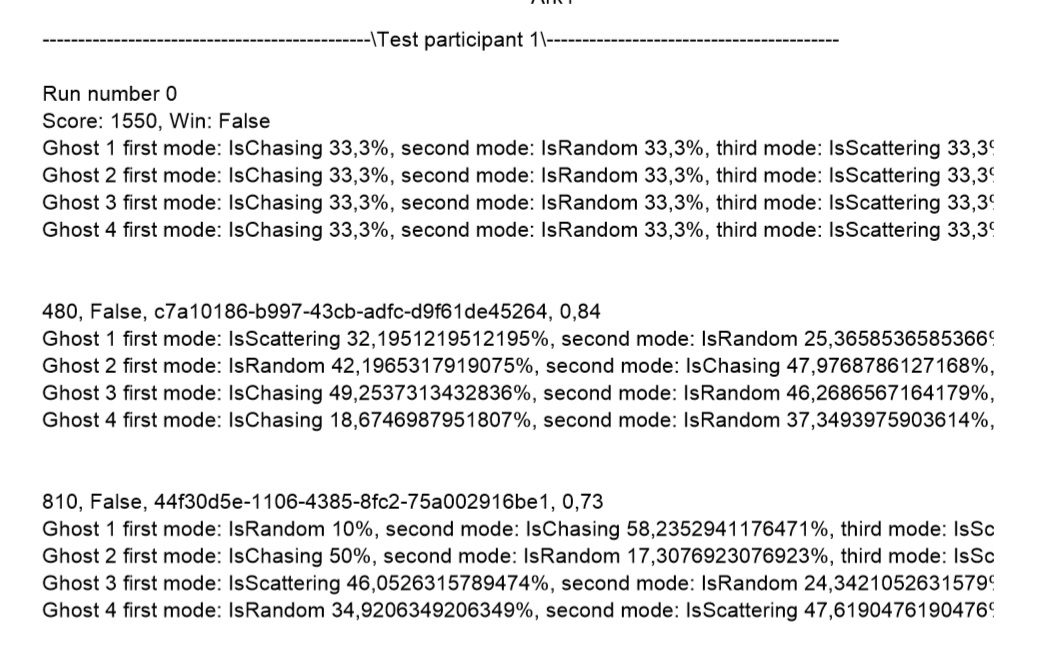
\includegraphics[scale=0.5]{testdata.jpg}
\caption{test data representation}
\label{fig:testdata}
\end{figure}


\newpage

The collected data consists of the following elements in descending order:

\begin{itemize}
\item  \textbf{Text participant}

Represent the participant number running from 1-21.
\item  \textbf{Run number}

Represent the current generation that the test participant is currently playing. Ranges from 0-9.
\item  \textbf{Score}

Represent the amount of points attained in the current generation/level.
\item  \textbf{Win}

Represent whether or not the test participant won the generation/level in a boolean statement. Win:True is the player won and Win:False is the player lost.
\item  \textbf{Ghost Mode}

Ghost 1-4 mode represent each of the four ghosts.


IsChasing, isRandom and isScattering represent the ghost Modes.(See section XX for mode description)

The percentages represent the length that each mode is active.

the order(sequence of modes) of each ghosts represent the order that the MonsterModes are switched between.(See section XX for documentation) Changing the order of the modes will change the time they are active during play or simulation in the prototype.
\end{itemize}

\newpage
Figure \ref{fig:testdata_simulation} depicts the data acquired of the simulations. After each level/generation played by a test participant there are 10 simulations.
The data recorded consists of the following elements for each simulation:

\begin{figure}[!htbp]
\centering
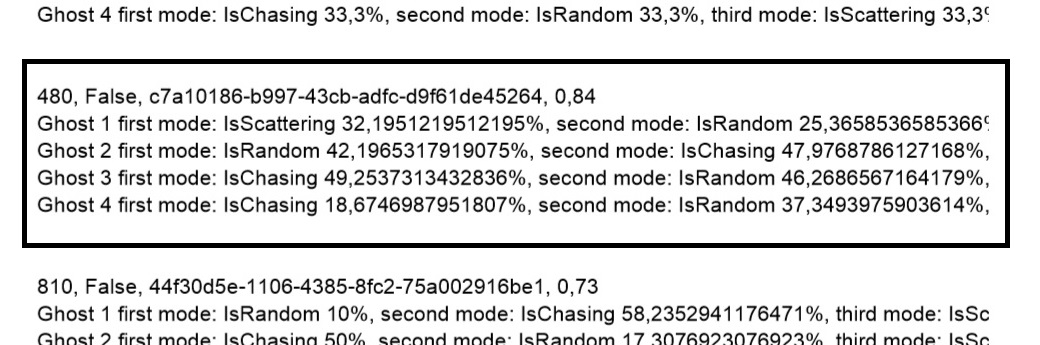
\includegraphics[scale=0.5]{testdata_simulation.jpg}
\caption{test data representation: Simulation}
\label{fig:testdata_simulation}
\end{figure}

\begin{itemize}
\item \textbf{first occurring number}

Represents the points collected during the entire simulation.

\item  \textbf{false/true}

Similar to the played level/generation, the boolean describes if the level is won or lost.

\item \textbf{<listCycles>}

The list represents the genes within each chromosome which are the solution to the given simulation.

\item \textbf{Fitness score}

The number ranging from 0-1 is the assigned fitness score to the current simulation. Depicted as 0.84 in the snippet(See figure \ref{fig:testdata_simulation})
\end{itemize}
\newpage
\subsubsection{Player level/generation points}
The following snippet(See figure \ref{fig:point_collection}) depicts the points collected by each one of the test participants from each generation/level.


The rows is the points collected from all test participants for each generation/level.

The columns are points collected by each test participant over the course of playing against the improved genetic algorithm over 10 generations. Ranging from generation 0 to generation 9(GEN 0 - GEN 9).
\begin{figure}[!htbp]
\centering
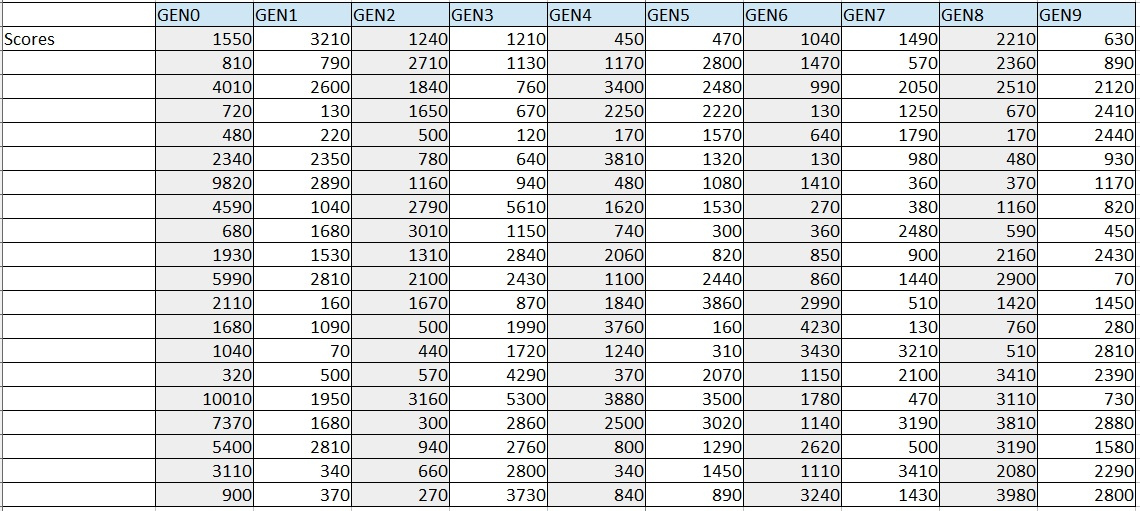
\includegraphics[scale=0.5]{player_points.jpg}
\caption{point collection}
\label{fig:point_collection}
\end{figure}

\newpage
\subsubsection{Questionnaire data}
The following data are the responses from the questionnaire acquired from the test participants.

\begin{itemize}
\item \textbf{How often do you play computer games?}
\begin{itemize}
\item 2 participants answered: never.
\item 6 test participants answered: Sometimes.
\item 5 test participants answered: Often.
\item 8 test participants answered: Very often.
\end{itemize}
\item \textbf{Please rate your skill in general computer/console games(scale from 1-10}

Figure \ref{fig:question2} represent the answer distribution on a scale from 1-10.

\begin{figure}[!htbp]
\centering
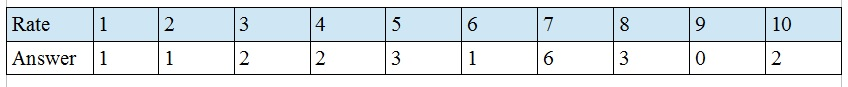
\includegraphics[scale=0.5]{question2.jpg}
\caption{test participant assessment of computer/console playing skill}
\label{fig:question2}
\end{figure}

\item \textbf{Are you familiar with the classic arcade game Pac-man}
\begin{itemize}
\item 21 test participants answered: Yes.
\item 0 test participants answered: No.
\end{itemize}
\item \textbf{If answering yes to the previous question, how often did/do you play it?}
\begin{itemize}
\item 5 test participants answered: Never.
\item 13 test participants answered: Sometimes.
\item 3 test participants answered: Often.
\item 0 test participants answered: Very often.
\end{itemize}
\item \textbf{Please rate your current skill level in the classic arcade game Pac-man(scale from 1-10)}

\begin{figure}[!htbp]
\centering
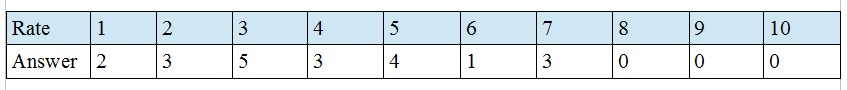
\includegraphics[scale=0.5]{question5.jpg}
\caption{test participant assessment of Pac-man playing skill}
\label{fig:question5}
\end{figure}

Figure \ref{fig:question5} represent the answer distribution on a scale from 1-10.


\end{itemize} 

\subsection{Result evaluation} \label{resulteval}





\subsection{Evaluation discussion}